\documentclass[twocolumn]{article}
\usepackage{graphicx}
\begin{document}
\title{Sine function}
\author{Wikipedia, the free encyclopedia}
\date{}
\maketitle

\begin{abstract}
A description of the sine function. From Wikipedia.
\end{abstract}

\section{Introduction}
In mathematics, the sine is a trigonometric function of an angle. The
sine of an acute angle is defined in the context of a right triangle:
for the specified angle, it is the ratio of the length of the side that
is opposite that angle to the length of the longest side of the triangle
(the hypotenuse).

More generally, the definition of sine (and other trigonometric functions)
can be extended to any real value in terms of the length of a certain line
segment in a unit circle. More modern definitions express the sine as an
infinite series or as the solution of certain differential equations,
allowing their extension to arbitrary positive and negative values and
even to complex numbers.

\begin{figure}[b]
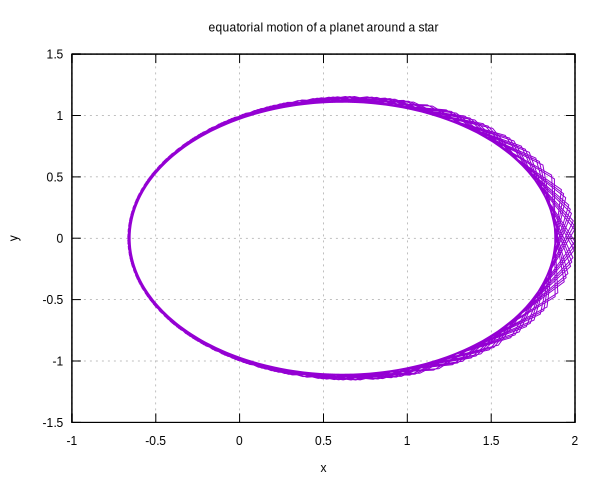
\includegraphics{plot.pdf}
\caption{Sine function}
\label{fig-sine}
\end{figure}

The sine function is commonly used to model periodic phenomena such as
sound and light waves, the position and velocity of harmonic oscillators,
sunlight intensity and day length, and average temperature variations
throughout the year.

The sine function is the solution to the following differential equation,
\begin{equation}
u''(x) = -u(x) \;,
\label{eq-sine-diff}
\end{equation}
with the initial condition
\begin{equation}
u(0)=0 \,,\; u'(0)=1 \;.
\label{eq-sine-iv}
\end{equation}

Here is a reference to Equation~(\ref{eq-sine-diff}). And
toEquation~(\ref{eq-sine-iv}). And a reference to the
Figure~(\ref{fig-sine}).

\end{document}